\documentclass[tikz]{standalone}

\usepackage{amsmath}
\usepackage[version=4]{mhchem}
\usepackage{siunitx}
% I only need the arrows for this one.
\usepackage{tikz}
\usetikzlibrary{arrows}

\begin{document}
    % New commands to keep things tidy.
    \newcommand{\Nu}[1]{\small $\nu_{#1}$}
    \newcommand{\Sig}[1]{$\sigma^{#1}$}
    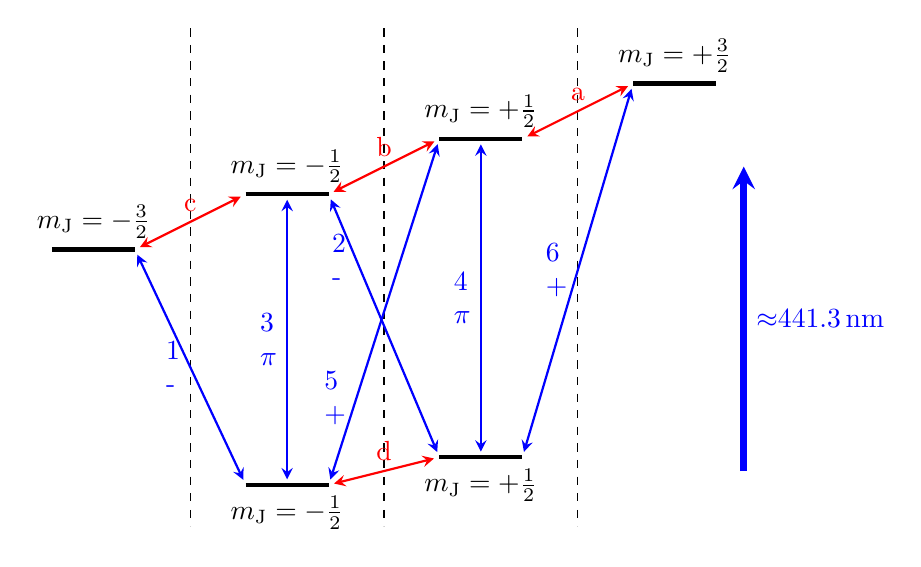
\begin{tikzpicture}[
        level/.style={ultra thick},
        separator/.style={dashed},
        optical trans/.style={blue, thick,<->,shorten >=2pt,shorten <=2pt,>=stealth},
        microwave trans/.style={red, thick,<->,shorten >=2pt,shorten <=2pt,>=stealth},
        laser/.style={blue, line width=0.25em,->,>=stealth}
    ]
        % Draw the energy levels.
        % 2P1/2
        \draw[level] (0em,-0.5em) -- ++(3em,0em) node[midway,below] {$m_\text{J}=-\frac{1}{2}$};
        \draw[level] (7em,0.5em) -- ++(3em,0em) node[midway,below] {$m_\text{J}=+\frac{1}{2}$};

        % 2P3/2
        \draw[level] (14em,14em) -- ++(3em,0em) node[midway,above] {$m_\text{J}=+\frac{3}{2}$};
        \draw[level] (7em,12em) -- ++(3em,0em) node[midway,above] {$m_\text{J}=+\frac{1}{2}$};
        \draw[level] (0em,10em) -- ++(3em,0em) node[midway,above] {$m_\text{J}=-\frac{1}{2}$};
        \draw[level] (-7em,8em) -- ++(3em,0em) node[midway,above] {$m_\text{J}=-\frac{3}{2}$};
        % draw angular momentum regions
        \draw[separator] (-2em,16em) -- (-2em,-2em);
        \draw[separator] (5em,16em) -- (5em,-2em);
        \draw[separator] (12em,16em) -- (12em,-2em);
        % Draw the optical transitions.
        \draw[optical trans] (0em,-0.5em) -- ++(-4em,8.5em) node[midway,left, align=left] {\Nu{1}\\\Sig{-}};
        \draw[optical trans] (7em,0.5em) -- ++(-4em,9.5em) node[near end,left, align=left] {\Nu{2}\\\Sig{-}};
        \draw[optical trans] (1.5em,-0.5em) -- ++(0em,10.5em) node[midway,left, align=left] {\Nu{3}\\$\pi$};
        \draw[optical trans] (8.5em,0.5em) -- ++(0em,11.5em) node[midway,left, align=left] {\Nu{4}\\$\pi$};
        \draw[optical trans] (3em,-0.5em) -- ++(4em,12.5em) node[near start,left, align=left] {\Nu{5}\\\Sig{+}};
        \draw[optical trans] (10em,0.5em) -- ++(4em,13.5em) node[midway,left, align=left] {\Nu{6}\\\Sig{+}};
        % Draw the microwave transitions.
        \draw[microwave trans] (10em,12em) -- ++(4em,2em) node[midway,above] {\Nu{a}};
        \draw[microwave trans] (3em,10em) -- ++(4em,2em) node[midway,above] {\Nu{b}};
        \draw[microwave trans] (-4em,8em) -- ++(4em,2em) node[midway,above] {\Nu{c}};
        \draw[microwave trans] (3em,-0.5em) -- ++(4em,1em) node[midway,above] {\Nu{d}};
        % Laser
        \draw[laser] (18em,0em) -- ++(0em,11em) node[midway,right] {\qty{\approx 441.3}{\nm}};
    \end{tikzpicture}
\end{document}
